% \chapter{Scenarios}\label{ch:scenarios}

% Delete the command below to remove the hints and instructions
\showscenariosnotes{}

\section{Scenarios}
    \todoinline{
	Illustrate how your architecture fulfills the most important data flows. As a rule of thumb, focus on the scenario of the assignment. Describe the scenario in terms of architectural components using UML Sequence diagrams and further explain the most important interactions in text. Illustrating the scenarios serves as a quick validation of the completeness of
	your architecture. If you notice at this point that for some reason, certain functionality or qualities are not addressed sufficiently in your architecture, it suffices to
	document this, together with a rationale of why this is the case according to you. You do not have to further refine you architecture at this point.
    }

    This section lists which sequence diagrams belong to which scenarios:
    \begin{itemize}
        \item UC11: Sensor data being processed by the system \\
              Figure \ref{fig:seq_scenario1}

        \item UC19: Subscribing to an application \\
              Figure \ref{fig:seq_scenario2}

        \item UC12: Applications issuing actuation commands \\
              Figure \ref{fig:seq_scenario3}

        \item UC14, Av3, UC18: Sensors/actuators failing \\
              Figure \ref{fig:seq_scenario4} \\
              This scenario displays the data flow when sensors/actuators fail, causing
              \begin{itemize}
                  \item deactivation of specific applications
                  \item a redundant sensor/actuator to take over in the context of a single application
              \end{itemize}

        \item Av2: Application crash \\
              Figure \ref{fig:seq_scenario5}

        \item U2, UC4: Plugging in a new pluggable device (sensor or actuator) \\
              Figure \ref{fig:seq_scenario6}

        \item Av1, UC15: Detection and handling of communication channel failure \\
              Figure \ref{fig:seq_scenario7}

        \item UC22, U1: Upgrading an application \\
              Figure \ref{fig:seq_scenario8}

        \item UC26, UC27, UC12: Sending actuation commands via a mobile app \\
              Figure \ref{fig:seq_scenario9}
    \end{itemize}

    \begin{figure}[!htp]
    	\centering
    	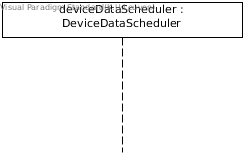
\includegraphics[width=\textwidth]{images/sequence-UC11}
    	\caption[Sensor data being processed by the system]{EXPLAIN WHAT HAPPENS IN THE SCENARIO. \\ ADD COMMENTS. \\ LINK TO OTHER RELEVANT SCENARIO'S. }\label{fig:seq_scenario1}
    \end{figure}

    \begin{figure}[!htp]
    	\centering
    	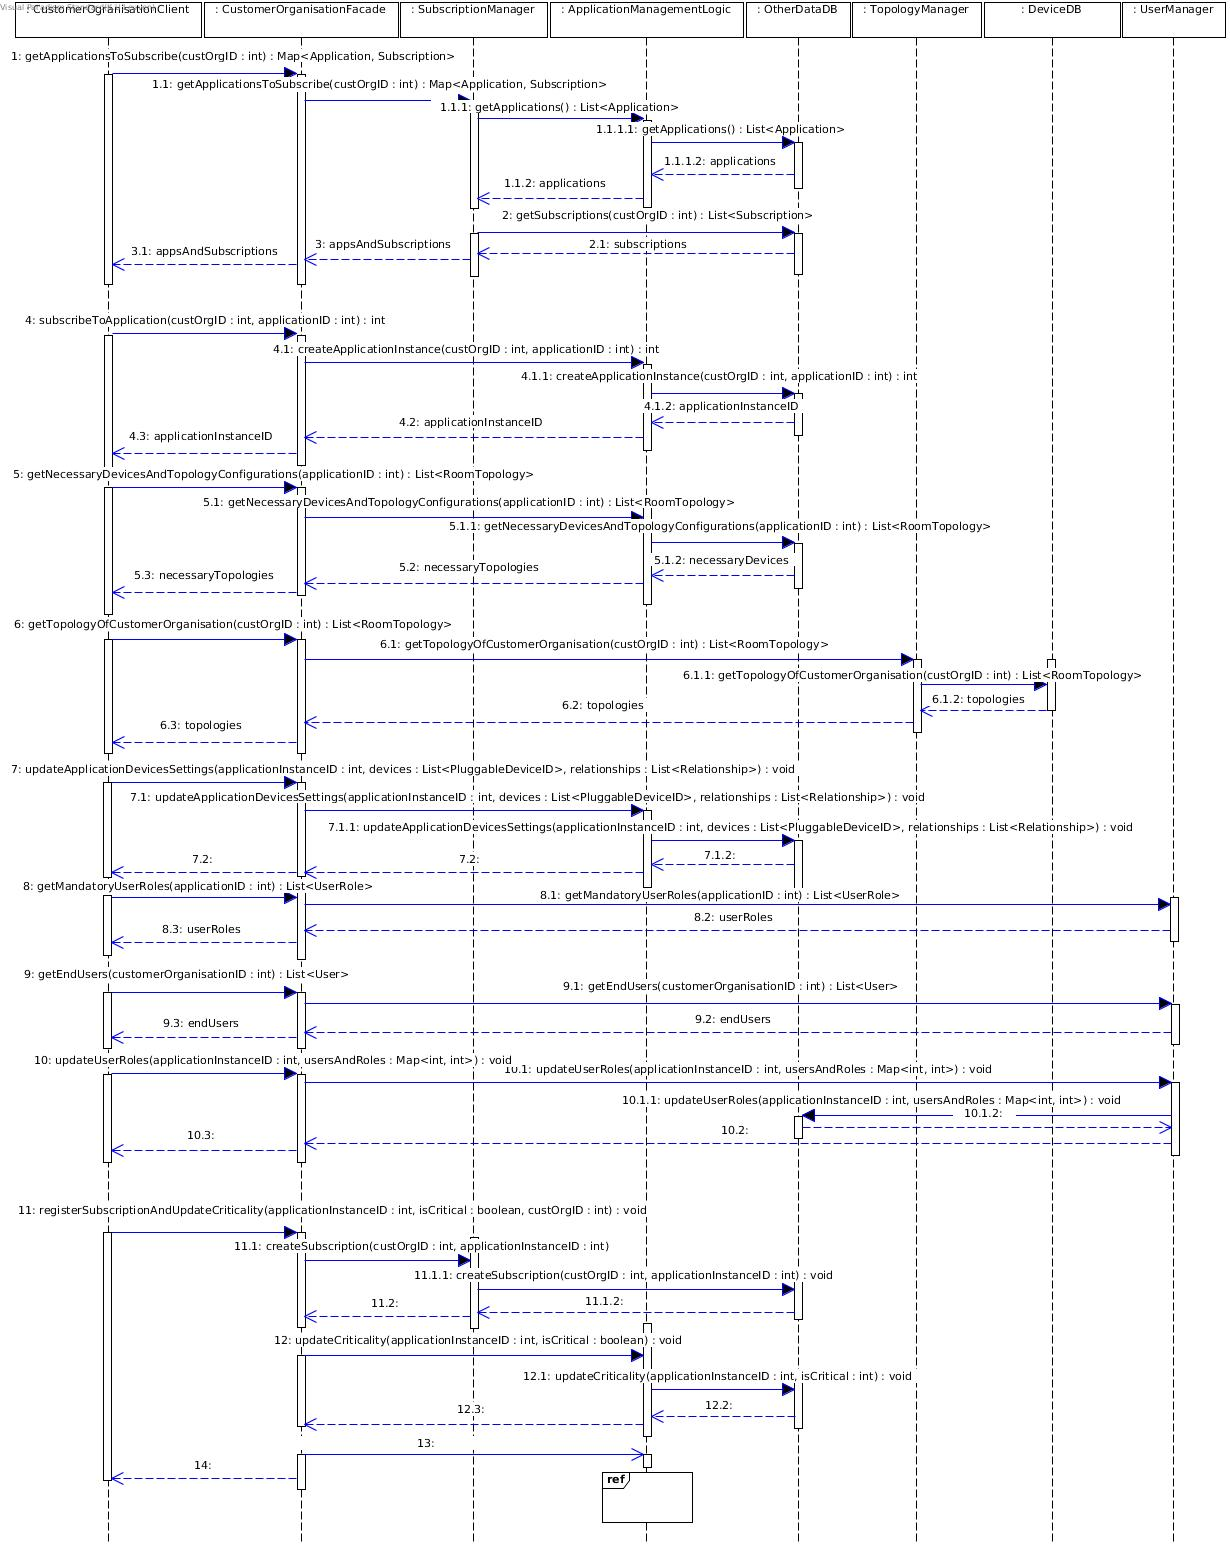
\includegraphics[width=\textwidth]{images/sequence-UC19}
    	\caption[ Subscribing to an application]{EXPLAIN WHAT HAPPENS IN THE SCENARIO. \\ ADD COMMENTS. \\ LINK TO OTHER RELEVANT SCENARIO'S. }\label{fig:seq_scenario2}
    \end{figure}

    \begin{figure}[!htp]
    	\centering
    	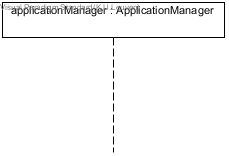
\includegraphics[width=\textwidth]{images/sequence-UC12}
    	\caption[Applications issuing actuation commands]{EXPLAIN WHAT HAPPENS IN THE SCENARIO. \\ ADD COMMENTS. \\ LINK TO OTHER RELEVANT SCENARIO'S. }\label{fig:seq_scenario3}
    \end{figure}

    \begin{figure}[!htp]
    	\centering
    	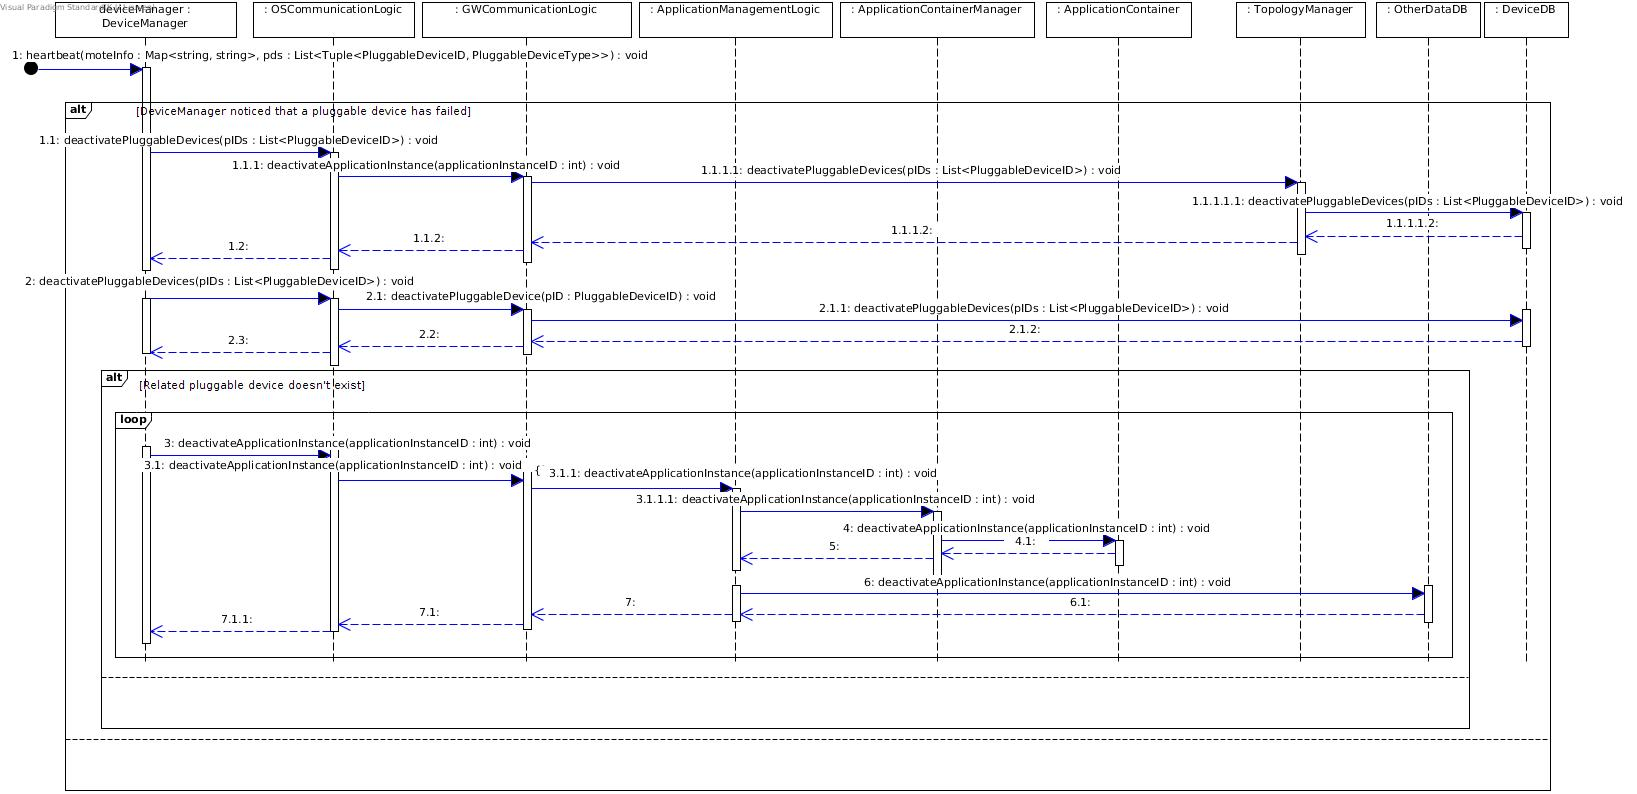
\includegraphics[width=\textwidth]{images/sequence-Av3-UC14-UC18}
    	\caption[Scenario ]{EXPLAIN WHAT HAPPENS IN THE SCENARIO. \\ ADD COMMENTS. \\ LINK TO OTHER RELEVANT SCENARIO'S. }\label{fig:seq_scenario4}
    \end{figure}

    \begin{figure}[!htp]
    	\centering
    	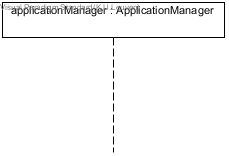
\includegraphics[width=\textwidth]{images/sequence-Av2}
    	\caption[Application crash]{EXPLAIN WHAT HAPPENS IN THE SCENARIO. \\ ADD COMMENTS. \\ LINK TO OTHER RELEVANT SCENARIO'S. }\label{fig:seq_scenario5}
    \end{figure}

    \begin{figure}[!htp]
    	\centering
    	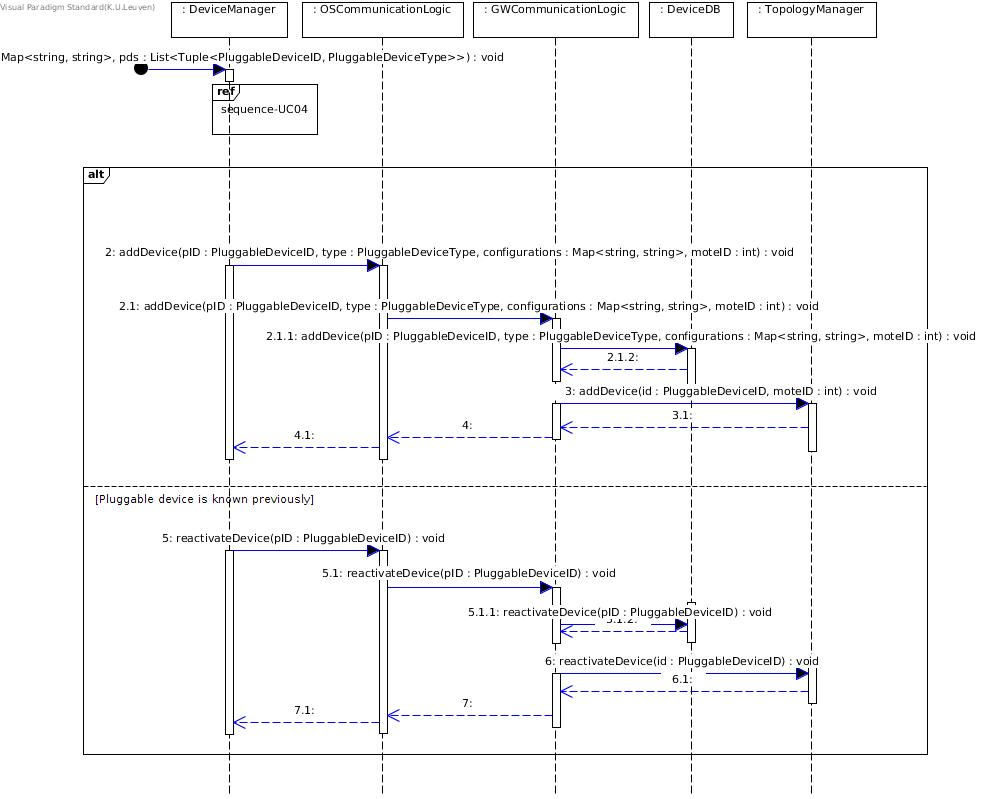
\includegraphics[width=\textwidth]{images/sequence-U2-UC4}
    	\caption[Plugging in a new pluggable device (sensor or actuator)]{EXPLAIN WHAT HAPPENS IN THE SCENARIO. \\ ADD COMMENTS. \\ LINK TO OTHER RELEVANT SCENARIO'S. }\label{fig:seq_scenario6}
    \end{figure}

    \begin{figure}[!htp]
    	\centering
    	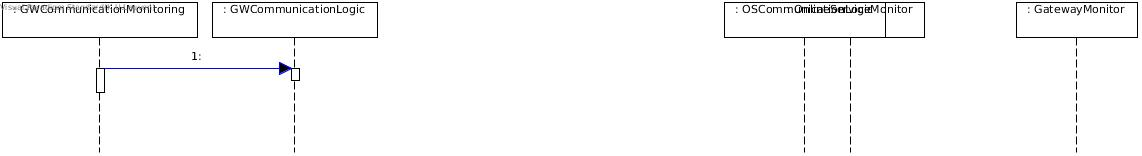
\includegraphics[width=\textwidth]{images/sequence-Av1-UC15}
    	\caption[Detection and handling of communication channel failure]{EXPLAIN WHAT HAPPENS IN THE SCENARIO. \\ ADD COMMENTS. \\ LINK TO OTHER RELEVANT SCENARIO'S. }\label{fig:seq_scenario7}
    \end{figure}

    \begin{figure}[h]
    	\centering
    	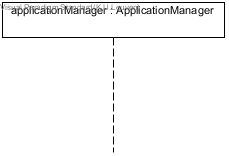
\includegraphics[width=\textwidth]{images/sequence-U1-UC22}
    	\caption[Upgrading an application]{EXPLAIN WHAT HAPPENS IN THE SCENARIO. \\ ADD COMMENTS. \\ LINK TO OTHER RELEVANT SCENARIO'S. }\label{fig:seq_scenario8}
    \end{figure}

    \begin{figure}[!htp]
    	\centering
    	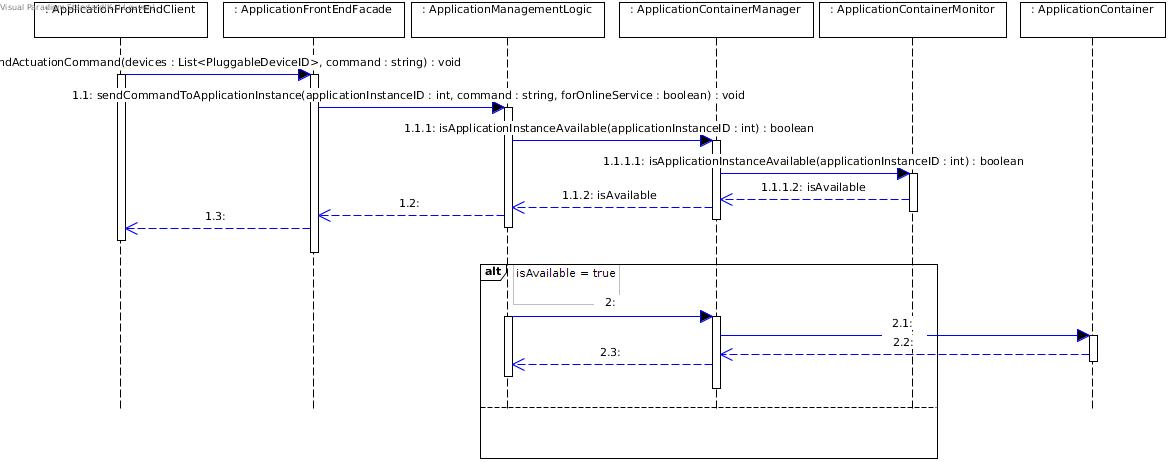
\includegraphics[width=\textwidth]{images/sequence-UC12-UC26-UC27}
    	\caption[Sending actuation commands via a mobile app]{EXPLAIN WHAT HAPPENS IN THE SCENARIO. \\ ADD COMMENTS. \\ LINK TO OTHER RELEVANT SCENARIO'S. }\label{fig:seq_scenario9}
    \end{figure}
